\chapter{FUNCTIONAL ANALYSIS AND MODELING}

Our approach is to transform the raw requirements collected from our stakeholders into functional models. The process is critically important for SmartExam as it works with low-level Windows API hooks, real-time telemetry, and WebSockets. Lack of clear boundary definition will cause the system to crash during a live, high load examination. Use-case tables and data flow diagrams are helpful in navigating this complexity.

The chapter is divided into 2 sections, the first deals with User Case modeling whereas the second section with Functional modeling. We begin with identifying our users and user stories to detail the different ways a Student, Teacher, and Administrator interact with the system, following this we present our data modeling by building an Entity Relationship Diagram and Data flow Diagrams to illustrate the data flow between client and back-end (ASP. Net Core).

\section{Use Case Modeling}

Use-case modeling is used for expressing the scope of the system from the end user's point of view \cite{uml_systems_analysis}. This allows us to focus on what the SmartExam system actually does, prior to the creation of code, and avoid ``scope creep'' as much as possible, so that both the student client, and teacher panel should remain on same page during implementation.

Our system consists of 3 Human actors: ``Student'', ``Teacher'', and ``Administrator''. It also has one automated Service Actor which is ``AI grader''. Figure~\ref{fig:usecase_diagram} shows the UML Use Case diagram for these roles.

\begin{figure}[H]
\centering
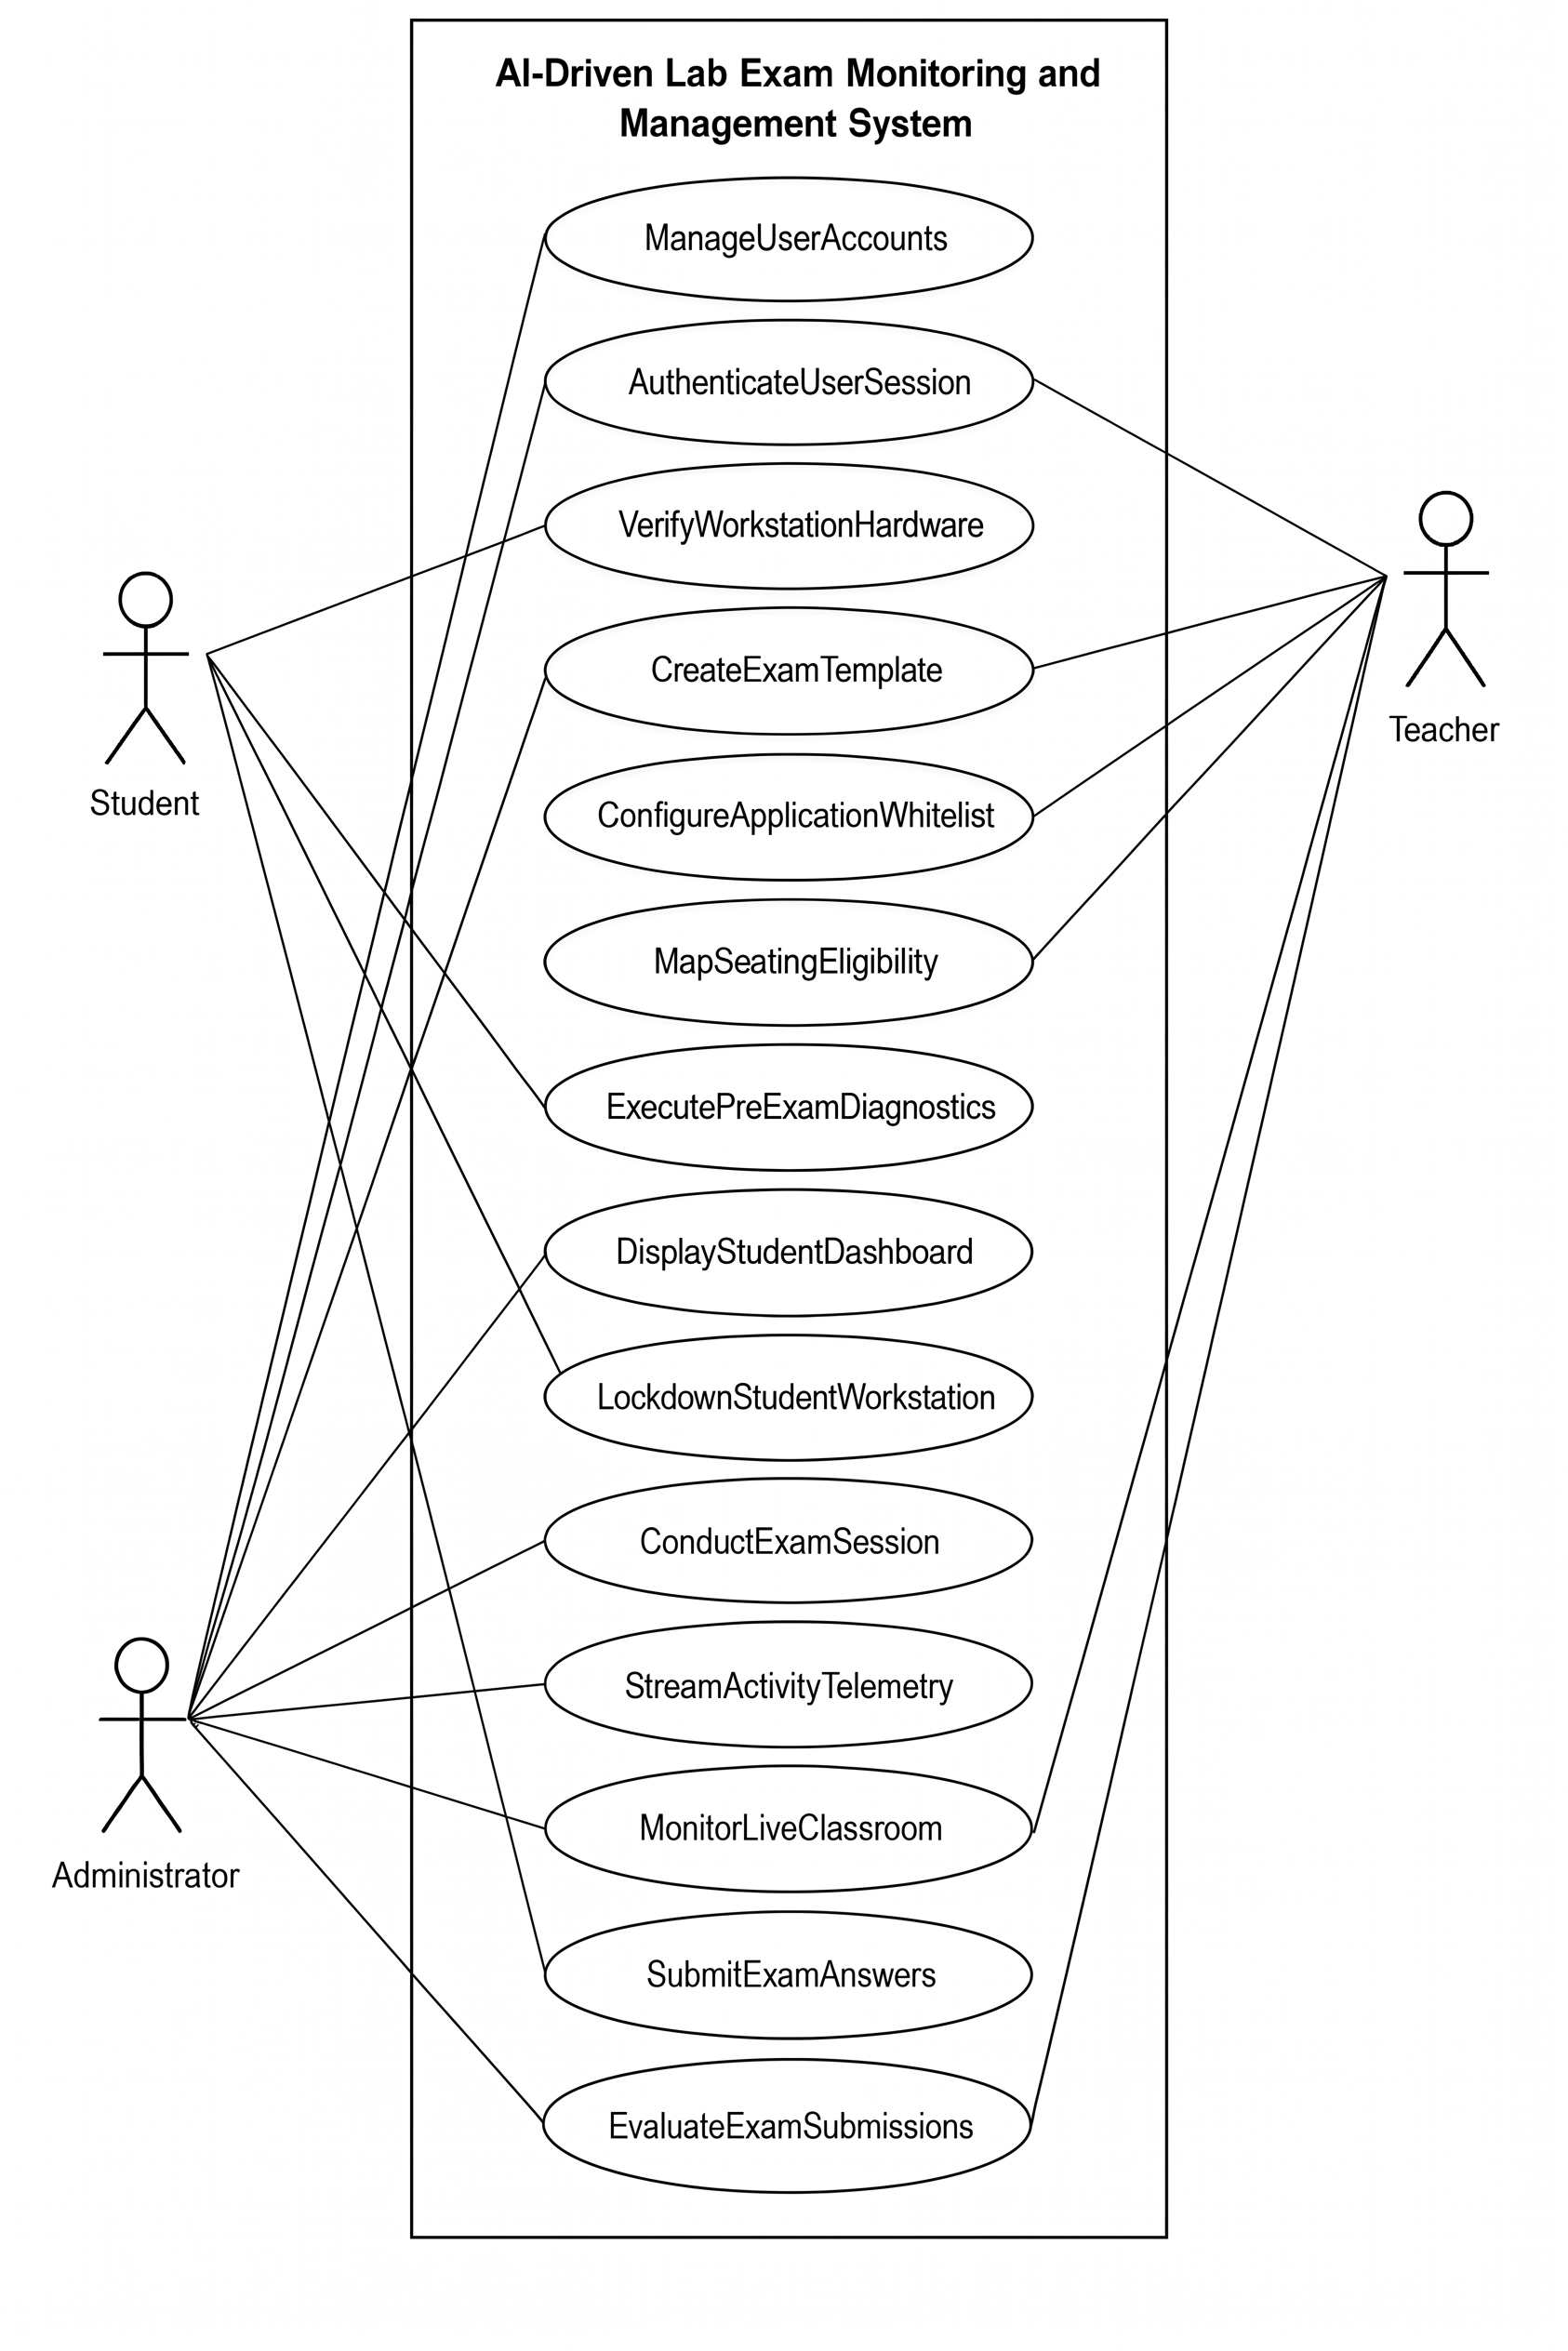
\includegraphics[width=0.55\linewidth]{Figures/use_case_diagram.png}
\caption{Use Case Diagram of the AI-Driven Lab Exam Monitoring System}
\label{fig:usecase_diagram}
\end{figure}

As shown in Figure~\ref{fig:usecase_diagram}, the roles are strictly separated. Students only access client-side features like hardware diagnostics and the exam environment. Teachers manage configurations, monitor WebSockets feeds, and review grading. Admins handle user profiles and audits. This strict separation helps us enforce security constraints at the database and API level.

\subsection{User Stories}

We wrote user stories to keep the Scrum team focused on user value \cite{user_stories_applied}. We used these stories to plan our sprints and define our done criteria.

The user stories for the AI-Driven Lab Exam Monitoring and Management System are organized by actor roles, covering the entire lifecycle of an examination from setup to monitoring, submission, evaluation, and reporting:

\subsubsection{Student User Stories}
\begin{enumerate}
    \item \textbf{Account Security:} As a student, I want to be prompted to create a secure password after initial account registration, so that my profile information is protected from unauthorized access.
    \item \textbf{Initial Setup and Biometric Enrollment (Optional):} As a student, I want the option to securely enroll biometric data (e.g., fingerprint, facial scan) during setup for enhanced login security, so that accessing the platform becomes quick and convenient while maintaining data integrity.
    \item \textbf{Pre-Exam Readiness Check:} As a student, I want the workstation client to perform a thorough pre-exam check, verifying the webcam, microphones, network connectivity, and essential system processes, so that I can confidently begin my examination knowing all configurations are optimal.
    \item \textbf{Mock Test Simulation:} As a student, I want to have access to short mock tests that mimic the locked-down environment and time constraints of the actual exam, so that I can familiarize myself with the restrictions and practice my problem-solving under simulated conditions.
    \item \textbf{Guided Exam Interface:} As a student, I want to be presented with a clear, intuitive exam interface displaying the countdown timer, current question, instructions, and the workspace clearly demarcated, so that I can focus on answering questions without confusion.
    \item \textbf{Lockdown Compliance:} As a student, I want the workstation client to automatically enforce lockdown restrictions by disabling Alt+Tab, the Windows key, and preventing the execution of unauthorized applications and external displays, so that I can concentrate on the exam and adhere to academic integrity standards.
    \item \textbf{Real-time Auto-Save:} As a student, I want my progress, including written answers and code, to be automatically saved to the server at frequent intervals (e.g., every 10 seconds), so that I am protected from data loss in case of system crashes or power outages.
    \item \textbf{Controlled and Forced Submission:} As a student, I want the option to manually submit my work before the timer expires, but also ensure that my completed exam is automatically submitted if I exceed the allowed time, so that my performance is accurately recorded for grading regardless of my actions.
\end{enumerate}

\subsubsection{Teacher User Stories}
\begin{enumerate}
    \item \textbf{Course and Exam Creation:} As a teacher, I want to easily create and manage courses, define exam templates with specific question types (coding, theoretical), durations, points, and set a grade percentage, so that I can structure my evaluations precisely.
    \item \textbf{Programming Environment Configuration:} As a teacher, I want to specify the allowed programming languages, libraries, and versions, and configure a whitelist of permitted desktop applications (e.g., specific IDEs, debuggers), so that students have the tools they need without unauthorized distractions.
    \item \textbf{Candidate Management and Scheduling:} As a teacher, I want to import student lists, assign them to specific exams, allocate them to particular labs or workstations, and set specific time windows for their participation, so that the exam process is organized and controlled.
    \item \textbf{Live Session Monitoring:} As a teacher, I want to have access to a real-time dashboard showing live status cards for each student, including their focus on the application, webcam feed, keyboard and mouse activity, and process list, so that I can effectively invigilate the class.
    \item \textbf{Violation Detection and Alerts:} As a teacher, I want to receive instant alerts for potential academic integrity violations, such as attempted task switching, execution of prohibited applications, or tampering with webcam feed, so that I can immediately address any issues.
    \item \textbf{Manual Invigilation Actions:} As a teacher, I want to have the ability to manually pause a student's exam timer, grant extensions, temporarily unlock their workstation for necessary assistance, or terminate a session if violations persist, so that I can manage special circumstances.
    \item \textbf{Automated Grading and Analysis:} As a teacher, I want the system to automatically compile coding submissions, run provided test cases, analyze theoretical answers for correctness and originality using semantic similarity checks, and identify instances of plagiarism, so that grading is efficient and accurate.
    \item \textbf{Performance Reporting and Auditing:} As a teacher, I want to generate comprehensive, exportable reports in PDF format that include student grades, invigilation logs (violations, extensions), AI grading feedback, and session summaries, so that I can review and archive assessment results.
\end{enumerate}

\subsubsection{Administrator User Stories}
\begin{enumerate}
    \item \textbf{User and Role Management:} As an administrator, I want to create, update, activate, and deactivate user accounts (students, teachers) and assign them specific roles with defined permissions, so that the system access is secure and aligns with institutional policies.
    \item \textbf{System Configuration and Setup:} As an administrator, I want to configure global system settings, including the IP address ranges for labs, default workstation parameters, database connection strings, and external service credentials, so that the system operates optimally across the institution.
    \item \textbf{Hardware Device Management:} As an administrator, I want to manage hardware device registrations and bindings, view their status, and have the ability to forcefully de-register devices if necessary, so that unauthorized hardware cannot be used for examinations.
    \item \textbf{Audit Trail Review:} As an administrator, I want to access and review detailed audit logs of critical system actions, such as user logins, role changes, system setting modifications, and invigilator overrides, so that I can ensure accountability and troubleshoot issues.
    \item \textbf{System Performance Monitoring:} As an administrator, I want to monitor key system performance metrics (CPU usage, memory, network traffic) on the server and client applications, so that I can proactively identify and address potential bottlenecks or issues.
    \item \textbf{Data Retention and Cleanup:} As an administrator, I want to configure policies for data retention and execute cleanup routines for old exam data, log files, and temporary files, so that the system's storage remains manageable.
\end{enumerate}

The user stories have been categorized to cover all 12 functional modules for AI-Driven Lab Exam Monitoring and Management System. The requirement for the student client, as well as the web panel, are addressed by these stories which allowed them to be developed in parallel within the agile sprints.

\subsection{Individual Actor Use Cases}

The user stories are expanded into detailed formal use case tables below. Each table depicts the necessary preconditions for a use case, triggers the use case, traces the primary flow, and presents the exception cases \cite{use_case_definition}. All tables use our unique project double-hline formatting.

Table~\ref{tab:uct_auth_device} describes the user authentication process. Using native Windows APIs, we read CPU, motherboard details from the client machine which form the HWID binding to prevent students login through any personal machine, or another machine in the lab, during the exam.

The Table~\ref{tab:uct_pre_exam_check} elaborates on the process to be done for each pre-exam check. We identify the status of the web cam, its connectivity and process list of the students along with its delay with our server. After all checks we record a baseline face of the student to compare it for authentication later.

Table~\ref{tab:uct_lockdown_telemetry} describes the locking down mechanism for the student's workstations. We use keyboard hooks at the low level to prevent use of Alt+Tab, Windows key and also block secondary monitor. We compress the screen shots from telemetric data to minimize the band width usage at random intervals.

Table~\ref{tab:uct_exam_config} focuses on exam setup features for a teacher. They have ability to upload code based tests and upload their respective Test cases along with other theory based questions, can configure applications that would be white-listed and select students to their assigned physical locations and IPs.

The Table~\ref{tab:uct_live_proctoring} demonstrates how the live session tracking by the teacher is designed. Live focus log and images is streamed from student clients to the teacher web dashboard using WebSockets. We color-coded user information at the teacher dashboard where Red indicates some lock-down violations, green signals for active usage.

Table~\ref{tab:uct_compilation_evaluation} explains the flow of automatic grading system. Each student's submitted code is first run inside a sand-boxed docker container, as they may contain a lot of infinite or blocking loops which can easily take down the backend server. Semantic similarity model is applied on theory answers.

Our Table~\ref{tab:uct_audit_report} demonstrates reporting capability of our system. After collection of all required data such as scores, HWIDs, web-socket based violations etc, we combine it into a single JSON payload, following which we call QuestPDF layout engine to produce a printable PDF document.

\begin{table}[H]
\centering
\caption{Use Case Table of User Authentication and Device Binding}
\label{tab:uct_auth_device}
\renewcommand{\arraystretch}{1.2}
\begin{tabular}{lp{10.6cm}}
\hline\hline
\textbf{Field} & \textbf{Details} \\
\hline\hline
\textbf{UCT ID} & UCT-01 \\
\textbf{Case Name} & Authenticate User and Verify Device Binding \\
\textbf{Overview} & Allows students to log in while validating their Hardware ID (HWID) to prevent proxy exam attempts. \\
\textbf{Actors} & Student, System (ASP.NET Core REST API) \\
\textbf{Pre-Conditions} & WPF client is running, network is active, and student profile is registered. \\
\textbf{Triggers} & Student launches the application and enters credentials on the login screen. \\
\textbf{Steps} & \begin{minipage}[t]{10.6cm}
1. Student enters registered email and password.\\
2. Client queries local APIs to fetch the unique workstation HWID.\\
3. Client transmits credentials and HWID to the REST API.\\
4. System validates credentials and compares HWID against stored binding.\\
5. System returns a secure JWT and redirects student to the dashboard.
\end{minipage} \\
\textbf{Post-Conditions} & The student is authenticated and device binding is verified. \\
\textbf{Exception Flow} & \begin{minipage}[t]{10.6cm}
1. Incorrect Credentials: System displays an error and prompts for retry.\\
2. HWID Mismatch: System blocks access and logs a security violation event.
\end{minipage} \\
\hline\hline
\end{tabular}
\end{table}

\begin{table}[H]
\centering
\caption{Use Case Table of Pre-Exam System Verification}
\label{tab:uct_pre_exam_check}
\renewcommand{\arraystretch}{1.2}
\begin{tabular}{lp{10.6cm}}
\hline\hline
\textbf{Field} & \textbf{Details} \\
\hline\hline
\textbf{UCT ID} & UCT-02 \\
\textbf{Case Name} & Perform Pre-Exam System Verification \\
\textbf{Overview} & Guides the student through hardware checks to ensure webcam, screen, and process compliance. \\
\textbf{Actors} & Student, System (WPF Client and REST API) \\
\textbf{Pre-Conditions} & Student is successfully authenticated and the exam session is scheduled. \\
\textbf{Triggers} & Student clicks ``Start Diagnostics'' on the client application interface. \\
\textbf{Steps} & \begin{minipage}[t]{10.6cm}
1. Client initializes and checks webcam, microphone, and screen sharing status.\\
2. Client scans active process lists for blacklisted applications.\\
3. Client performs a network connection latency and bandwidth test.\\
4. Client prompts the student to capture a webcam reference snapshot.\\
5. Client uploads diagnostics status and reference photo to the server.
\end{minipage} \\
\textbf{Post-Conditions} & Diagnostics logs are stored and student is cleared to launch the exam workspace. \\
\textbf{Exception Flow} & \begin{minipage}[t]{10.6cm}
1. Diagnostic Failure: System flags errors and disables the exam launch button.\\
2. Blocked Process: Client lists running blacklisted apps and prompts user to close them.
\end{minipage} \\
\hline\hline
\end{tabular}
\end{table}

\begin{table}[H]
\centering
\caption{Use Case Table of Workstation Lockdown and Telemetry Tracking}
\label{tab:uct_lockdown_telemetry}
\renewcommand{\arraystretch}{1.2}
\begin{tabular}{lp{10.6cm}}
\hline\hline
\textbf{Field} & \textbf{Details} \\
\hline\hline
\textbf{UCT ID} & UCT-03 \\
\textbf{Case Name} & LOCKDOWN WORKSTATION AND STREAM TELEMETRY \\
\textbf{Overview} & RESTRICTS DESKTOP TASK-SWITCHING AND STREAMS PERIODIC SCREENSHOTS AND LOGS TO THE SERVER. \\
\textbf{Actors} & STUDENT, SYSTEM (WPF CLIENT AND REST API) \\
\textbf{Pre-Conditions} & STUDENT HAS PASSED DIAGNOSTICS, AND THE SCHEDULED EXAM SESSION IS LAUNCHED. \\
\textbf{Triggers} & STUDENT LAUNCHES THE LOCKED EXAM SCREEN. \\
\textbf{Steps} & \begin{minipage}[t]{10.6cm}
1. CLIENT ENTERS FULLSCREEN MODE AND BLOCKS HOTKEYS (ALT+TAB, WIN KEY) VIA HOOKS.\\
2. CLIENT DETECTS AND DISABLES SECONDARY MONITOR CONNECTIONS.\\
3. CLIENT STARTS BACKGROUND THREADS TO MONITOR ACTIVE PROCESSES AND FOCUS STATES.\\
4. CLIENT CAPTURES SCREENSHOTS AT RANDOMIZED INTERVALS (30 TO 90 SECONDS).\\
5. CLIENT PACKAGES AND STREAMS FOCUS LOGS AND SCREENSHOTS TO THE SERVER VIA WEBSOCKET.
\end{minipage} \\
\textbf{Post-Conditions} & WORKSTATION REMAINS LOCKED, AND TELEMETRY DATA IS CONTINUOUSLY SAVED. \\
\textbf{Exception Flow} & \begin{minipage}[t]{10.6cm}
1. LOCKDOWN BYPASS: CLIENT DETECTS HOOK EVASION, SOUNDS AN ALARM, AND LOCKS SCREEN.\\
2. NETWORK INTERRUPTION: CLIENT CACHES TELEMETRY IN ENCRYPTED LOCAL STORE.
\end{minipage} \\
\hline\hline
\end{tabular}
\end{table}

\begin{table}[H]
\centering
\caption{Use Case Table of Exam Configuration and Access Control}
\label{tab:uct_exam_config}
\renewcommand{\arraystretch}{1.2}
\begin{tabular}{lp{10.6cm}}
\hline\hline
\textbf{Field} & \textbf{Details} \\
\hline\hline
\textbf{UCT ID} & UCT-04 \\
\textbf{Case Name} & Configure Exam and Seating Access Controls \\
\textbf{Overview} & Enables teachers to design exam templates, whitelists, and map laboratory seating. \\
\textbf{Actors} & Teacher, System (React Admin Panel and REST API) \\
\textbf{Pre-Conditions} & Teacher is authenticated and has administrative rights over the course. \\
\textbf{Triggers} & Teacher selects ``Create New Exam'' on the web-based console. \\
\textbf{Steps} & \begin{minipage}[t]{10.6cm}
1. Teacher enters exam metadata, questions, and allowed application whitelist.\\
2. Teacher uploads public and hidden test cases for coding tasks.\\
3. Teacher configures proctoring levels (screenshot intervals, webcam checks).\\
4. Teacher maps candidate registrations to physical lab IP ranges and seat IDs.\\
5. Teacher publishes the configuration to the central database.
\end{minipage} \\
\textbf{Post-Conditions} & The exam template is created, access policies are set, and the exam is scheduled. \\
\textbf{Exception Flow} & \begin{minipage}[t]{10.6cm}
1. Formatting Error: System flags failing test case syntax and requests correction.\\
2. Seating Conflict: System displays collision warnings for overlapping mappings.
\end{minipage} \\
\hline\hline
\end{tabular}
\end{table}

\begin{table}[H]
\centering
\caption{Use Case Table of Live Proctoring and Violation Alerting}
\label{tab:uct_live_proctoring}
\renewcommand{\arraystretch}{1.2}
\begin{tabular}{lp{10.6cm}}
\hline\hline
\textbf{Field} & \textbf{Details} \\
\hline\hline
\textbf{UCT ID} & UCT-05 \\
\textbf{Case Name} & MONITOR LIVE PROCTORING AND HANDLE ALERTS \\
\textbf{Overview} & PROVIDES TEACHERS WITH A LIVE DASHBOARD OF STUDENT STATUSES, LOGS, AND VIOLATION ALERTS. \\
\textbf{Actors} & TEACHER, SYSTEM (REACT ADMIN PANEL, WEBSOCKET HUB) \\
\textbf{Pre-Conditions} & THE EXAM SESSION IS ACTIVE, AND STUDENTS ARE LOGGED IN VIA THE WPF CLIENT. \\
\textbf{Triggers} & TEACHER ACCESSES THE ACTIVE EXAM MONITORING DASHBOARD. \\
\textbf{Steps} & \begin{minipage}[t]{10.6cm}
1. DASHBOARD ESTABLISHES A SECURE WEBSOCKET LINK TO THE CENTRAL SERVER.\\
2. DASHBOARD DISPLAYS A VISUAL GRID OF ACTIVE STUDENT STATUS CARDS.\\
3. SYSTEM PUSHES REAL-TIME TELEMETRY LOGS AND ALERTS TO THE DASHBOARD.\\
4. TEACHER VIEWS LOGS, SCREENSHOTS, AND ACTIVE PROCESSES FOR FLAGGED STUDENTS.\\
5. TEACHER RESOLVES ALERTS OR ISSUES MANUAL OVERRIDES (PAUSE TIMER, FORCE SUBMIT).
\end{minipage} \\
\textbf{Post-Conditions} & THE TEACHER MAINTAINS OVERSIGHT, AND ALERTS ARE RESOLVED OR ACTED UPON. \\
\textbf{Exception Flow} & \begin{minipage}[t]{10.6cm}
1. CONNECTION LOST: DASHBOARD DISPLAYS OFFLINE STATUS AND ATTEMPTS TO RECONNECT.\\
2. STUDENT DISCONNECTS: GRID CARD MARKS STUDENT AS OFFLINE AND FLAGS A WARNING.
\end{minipage} \\
\hline\hline
\end{tabular}
\end{table}

\begin{table}[H]
\centering
\caption{Use Case Table of Process Code Compilation and Evaluation}
\label{tab:uct_compilation_evaluation}
\renewcommand{\arraystretch}{1.2}
\begin{tabular}{lp{10.6cm}}
\hline\hline
\textbf{Field} & \textbf{Details} \\
\hline\hline
\textbf{UCT ID} & UCT-06 \\
\textbf{Case Name} & PROCESS CODE COMPILATION AND SEMANTIC EVALUATION \\
\textbf{Overview} & AUTOMATICALLY COMPILES PROGRAMMING TASKS, GRADES THEORY QUESTIONS VIA AI, AND CHECKS PLAGIARISM. \\
\textbf{Actors} & SYSTEM (REST API AND AI GRADING MICROSERVICE), TEACHER \\
\textbf{Pre-Conditions} & STUDENTS HAVE SUBMITTED THEIR EXAMS, AND THE GRADING PHASE IS INITIATED. \\
\textbf{Triggers} & SYSTEM RECEIVES AN EXAM SUBMISSION OR TEACHER INITIATES AUTO-GRADING. \\
\textbf{Steps} & \begin{minipage}[t]{10.6cm}
1. SYSTEM PULLS SUBMITTED CODE AND THEORY ANSWERS FROM THE DATABASE.\\
2. SYSTEM COMPILES CODE INSIDE ISOLATED CONTAINERS AGAINST TEST CASES.\\
3. SYSTEM SENDS THEORY ANSWERS TO THE AI SEMANTIC ENGINE FOR EVALUATION.\\
4. SYSTEM RUNS PLAGIARISM ANALYSIS ACROSS ALL STUDENT FILES.\\
5. SYSTEM CONSOLIDATES SCORES AND PLAGIARISM FLAGS INTO A GRADE SHEET.
\end{minipage} \\
\textbf{Post-Conditions} & SUBMISSIONS ARE COMPILED, AI SEMANTIC GRADES ARE COMPUTED, AND MARKS ARE SAVED. \\
\textbf{Exception Flow} & \begin{minipage}[t]{10.6cm}
1. COMPILATION ERROR: CODE IS RECORDED WITH ZERO TEST PASS SCORE AND ERROR DETAILS.\\
2. AI SERVICE OFFLINE: SYSTEM CACHES REQUESTS AND FLAGS QUESTIONS AS PENDING REVIEW.
\end{minipage} \\
\hline\hline
\end{tabular}
\end{table}

\begin{table}[H]
\centering
\caption{Use Case Table of Audit Logging and Report Export}
\label{tab:uct_audit_report}
\renewcommand{\arraystretch}{1.2}
\begin{tabular}{lp{10.6cm}}
\hline\hline
\textbf{Field} & \textbf{Details} \\
\hline\hline
\textbf{UCT ID} & UCT-07 \\
\textbf{Case Name} & GENERATE AUDIT LOGS AND EXPORT REPORTS \\
\textbf{Overview} & RECORDS SYSTEM EVENTS AND EXPORTS ATTENDANCE, GRADES, AND VIOLATION LOGS AS A PDF REPORT. \\
\textbf{Actors} & TEACHER, ADMINISTRATOR, SYSTEM \\
\textbf{Pre-Conditions} & THE EXAM SESSION HAS CONCLUDED, AND GRADING REVIEWS ARE FINALIZED. \\
\textbf{Triggers} & TEACHER OR ADMIN CLICKS ``EXPORT SESSION PDF'' ON THE DASHBOARD. \\
\textbf{Steps} & \begin{minipage}[t]{10.6cm}
1. SYSTEM QUERIES DATABASE FOR ATTENDANCE, HWIDS, SCORES, AND VIOLATION EVENTS.\\
2. SYSTEM EXTRACTS IMMUTABLE AUDIT LOGS OF ADMINISTRATOR AND TEACHER OVERRIDES.\\
3. SYSTEM PACKAGES DATA INTO JSON AND INVOKES THE QUESTPDF ENGINE.\\
4. QUESTPDF GENERATES A STYLED PDF DOCUMENT WITH SCORE CHARTS AND TIMELINES.\\
5. SYSTEM LOGS THE EXPORT EVENT AND DOWNLOADS THE PDF TO THE USER'S BROWSER.
\end{minipage} \\
\textbf{Post-Conditions} & A SECURE, STYLED PDF REPORT IS DOWNLOADED AND THE EVENT IS LOGGED. \\
\textbf{Exception Flow} & \begin{minipage}[t]{10.6cm}
1. DATA INCONSISTENCY: SYSTEM DISPLAYS ERROR DETAILS AND LOGS A CRITICAL WARNING.\\
2. MISSING RECORDS: SYSTEM GENERATES THE REPORT WITH EMPTY FIELDS FOR MISSING DATA.
\end{minipage} \\
\hline\hline
\end{tabular}
\end{table}
